\documentclass[11pt,a4paper,titlepage]{article}
\PassOptionsToPackage{hyphens}{url}\usepackage{hyperref}
\usepackage[margin=1in]{geometry}
\usepackage[page]{appendix}
\usepackage[nottoc]{tocbibind}
\usepackage{graphicx}
\usepackage[ruled,vlined, linesnumbered]{algorithm2e}
\graphicspath{{./images/}}

\author{Alex Campbell}
\date{}

\begin{document}

\setlength{\parindent}{0em}
\setlength{\parskip}{1em}

\section*{Abstract}

\pagebreak
\tableofcontents
\pagebreak

\section{Introduction}
The Travelling Salesperson Problem (TSP) is an NP-Hard problem which is commonly found in combinatorial optimisation, theoretical computer science and operations research. It's a simple problem on the surface which simply states that "Given a list of cities and distances between each pair of them, what is the shortest possile route that visits each city exactly once and returns to the origin city?" \cite{TSPWiki}

This question appears deceptively simple, however with large sets of cities the search space becomes incredibly large, and as such computation time can be astronomical, since before you even start trying to compute the shortest tour, there are n! different combinations to compute, assuming a complete graph. Clearly this meant another angle had to be taken for this problem.

As such many people decided to go for a more heuristic approach towards solving the TSP problem. So instead of trying to find the optimal solution with an infeasibly long time span, we would settle for a 'good enough' solution with a much lower time complexity, however since TSP is a combinatorial optimisation problem it is much more difficult than continuous optimisation, with higher chances of falling into local optimum rather than the global optimum.

And yet even with this said, there exists an algorithm that has been created more than 30 years ago (1976) that has been proven to be at most 50\% worse than the optimal solution for any given TSP problem and is known as Christofides algorithm. This algorithm has remained the best approximation available for over 30 years, and only recently in this year (2020) has another, slightly more efficient algorithm been found \cite{TSP2020}, although it has yet to be verified even if the general consensus is that it seems correct.

However another way of finding approximate solutions is becoming more and more popular over time, and has its roots deeply set in evolution and natural selection, hence the name they are given: Evolutionary algorithms. In essence these algorithms replicate the generational aspect of natural selection, taking the best individuals from a given population and 'breeding' them, these 'children' can then be tested to see if they perform any better than their parents, and if so replace the worst individuals in the population, and this process continues to repeat until a given goal is complete, whether that turns out to be an actual solution being found, until a good enough solution is found or after a certain number of generations have been looped through.

Genetic algorithms have already been used to try and solve the TSP which shall be discussed later, yet the major point of genetic algorithms is that you start with an entirely random population with which to create new solutions with a large degree of randomness in terms of the search operators. If however we were to replace one of the population with a strong approximate solution ($x$), how would that affect the algorithm? Theoretically in the worst case scenario this genetic algorithm would simply return $x$, since if no better one can be found, then $x$ would remain in the population as the best solution, so we are no worse off compared to when we started the algorithm. However in the best case scenario the algorithm would produce a better approximate solution than $x$ and return this instead.

As such, in this thesis I will be investigating the usage of both the mathematical and algorithmic methods of finding a solution to the Travelling Salesman Problem, and thereby seeing if these methods can be combined into a singular algorithm that can find a more optimal solution.

\section{Background}

\subsection{Christofides Algorithm}
Even with the algorithm having been created over 30 years ago in 1976, there has yet to be another verified algorithm at this time that can produce more optimal approximate solutions to the TSP problem than this. This algorithm has been proven to be at most 50\% worse than the optimal solution whilst having an $O(n^3)$ time complexity where n is the number of cities for which we are trying to solve the problem. \cite{ChrAlg} If we instead look at the best algorithm currently available to solve the TSP (aka the Held-Karp Algorithm) we can see that its complexity is $O(n^2 2^n)$ \cite{HeldKarpAlg} which, whilst astronomically better than the original $O(n!)$, is significantly worse than the approximate solution that Christofides algorithm provides.

This is often the case with such computationally expensive problems, a balance must often be made between finding the optimal solution, and finding a solution in an appropriate amount of time. The Held-Karp algorithm focuses more on finding the optimum answer rather than finding it in a feasible amount of time, whereas Christofides Algorithm was designed to find as best an approximation as it can whilst still having a relatively feasible computation time which is what can make it so appealing to use. 

One of the strong points about Christofides algorithm is just how simple it is, having only 4 or 5 major steps (many sources combine steps 4 and 5 whilst others do not \cite{ChrAlgSlides, ChrAlgSteps}) even if these steps are more likes processes themselves. 

Nonetheless the steps to this algorithm are as follows:
\begin{enumerate}
	\item Find a minimum spanning tree $T$.
	\item Find a minimum weight perfect matching $M$ for the odd degree vertices in $T$.
	\item Calculate $M \bigcup T$.
	\item Find an Euler tour of $M \bigcup T$.
	\item Remove any repeated vertices.
\end{enumerate}

\begin{figure}[ht]
	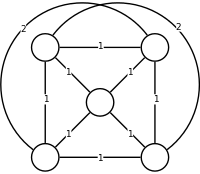
\includegraphics[scale=0.75]{WikiCompleteGraph}
	\centering
	\caption{Full Graph}
\end{figure}

\clearpage
As stated the process is compressed into few steps and is quite simple to understand, and yet creating this algorithm within a programming language is more complex than one would initially assume. Finding a minimum spanning tree (Figure 2) of the full graph (Figure 1) is quite simple, the two most common algorithms known for solving this are Prims and Kruskals, both of which are effective methods with time complexities of $O(n)$ and $O(n^2)$ respectively \cite{PvKTime} though choosing one or the other is mostly affected by the number of edges within the graph we are finding the minimum spanning tree for, with Prims being more suitable if there are a large number of edges, and Kruskals if not.

\begin{figure}[ht]
	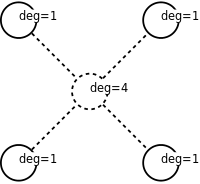
\includegraphics[scale=0.6]{WikiMinSpanTree}
	\centering
	\caption{Minimum Spanning Tree}
\end{figure}

The minimum weight perfect matching of $T$ (Figure 3) is accomplished by finding $\frac{T}{2}$ edges which 'link' together every vertex in $T$ by the shortest edge possible. For this one of the most common algorithm in use appears to be the blossom algorithm and has a time complexity of $O(n^2 m)$ in the worst case where $n$ is the number of vertices and $m$ is the number of edges \cite{BlosAlg}.

\begin{figure}[ht]
	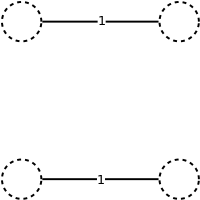
\includegraphics[scale=0.6]{WikiMinMatch}
	\centering
	\caption{Minimum Weight Perfect Matching}
\end{figure}

From here we simply calculate the union of $M$ and $T$ (Figure 4), including any of the repeated edges that may be present, before moving onto the Euler tour. A Euler tour is simply a tour of the graph which visits each edge exactly once, regardless of starting or ending vertex (Figure 5).

\begin{figure}[ht]
	\centering
		\begin{minipage}{0.45\textwidth}
			\centering
			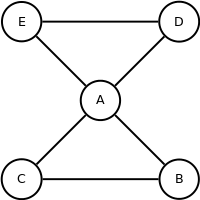
\includegraphics[scale=0.5]{WikiComb}
			\caption{$M \bigcup T$}
		\end{minipage}\hfill
		\begin{minipage}{0.45\textwidth}
			\centering
			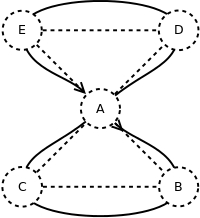
\includegraphics[scale=0.5]{WikiEulerTour}
			\caption{Euler Tour}
		\end{minipage}\hfill
\end{figure}

Then need to remove any repeated vertices within our tour and replace them with the direct edge between those vertices, and once this is done we have the algorithms output (Figure 6).

\begin{figure}[ht]
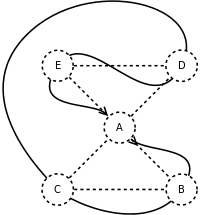
\includegraphics[scale=0.6]{WikiRemove}
\centering
\caption{Christofides Algorithm Output}
\end{figure}

(Figures 1-6 taken from: Wikipedia: Travelling Saleman Problem \cite{TSPWiki})

With this algorithm output we now have a solution to the TSP for our specific graph, and this solution is guaranteed to be within 50\% of the optimum \cite{ChrAlg}, which is significantly better than trying to calculate the true optimum for a very large graph in an infeasible amount of time. However there is clear room for improvement, hence why other methods have been designed and tested.

\subsection{Genetic Algorithms}
Genetic algorithms take deep inspiration from natural selection and evolution in general. The very simplest description of a genetic algorithm is that given a starting population of predetermined size, calculate the fitness of each individual and choose the best of the population to 'reproduce' to create individuals that theoretically have the genes of both of these individuals, potentially giving it a higher fitness than its two parents. This child then has its fitness evaluated and if it is better than the worst individual in the population, it is added in place of it, this repeats for as many generations as we have chosen, and at the end of it we have a population of individuals who may have a better overall fitness than the initial population.

Most genetic algorithms take a very similar form, and though it is often altered for each individual case it is used in, most look very similar to the following pseudocode \cite{GAIntro}.
\clearpage

\begin{algorithm}[H]
\SetAlgoLined
\textbf{Initial Values:} generationNum = 0, generationMax = $N$\footnote{Where $N$ is a predetermined number of generations}\;
Randomly generate a population of size $P$ individuals to be used initially\;
Calculate the fitness of all $P$ individuals\;
Sort the algorithm in descending order of fitness\;
\While{(generationNum $<$ generationMax)}{
	Pick the $M$\footnote{$ 2 \leq M \leq P$} best individuals from the start of the population\;
	\For{(each pair of parents in $M$\footnote{Selected randomly with replacement})}{
		Apply the crossover and mutation operators to produce two new offspring\;
		Evaluate their fitness\;
	}
	Replace the worst individuals in the population with the offspring assuming said offspring have a higher fitness than them \footnote{If all of the population are used to create new individuals then it will be the case that the entire population is replaced.}\;
	generationNum += 1\;
}
\caption{Pseudocode for a basic Genetic Algorithm}
\end{algorithm}

From the pseudocode it is most likely very clear that genetic algorithm is very well suited for optimisation problems, either maximising or minimising the fitness of the individuals in the population. This means it is definitely a viable option to solve the TSP, since the entire purpose of that is to minimise the weight of the path through all of the cities. However the pseudo code also shows there are a few operators and functions that need to be defined and explained before anything fruitful can be done.

\subsubsection{Individuals}

More of a clarification point more than anything, we need to decide what the individuals actually are within our problem of the TSP. Simply enough these individuals are solutions to the TSP, that is they are all routes that pass through each city and end back at the starting point, all without visiting a given city twice. The more important part however is how these routes should be stored in a way that the computer can work with, since naturally a picture of the route, whilst technically plausible, would be far more hassle than it would be worth given there exists much simpler encoding methods.

Given that a solution to the TSP requires that all cities within $C$ be used, a solution can simply be seen as an arrangement of these cities, whether this be as an array, list or simply a string. Any one of these formats would be suitable and effective to allow for the crossover and mutation functions to be applied, since regardless of format, all solutions will be of the same size.

\subsubsection{Objective Function and Fitness}

As stated briefly before, the TSP is an optimisation problem at its core, and genetic algorithms are powerful at solving such problems, and since this is a single objective optimisation problem in this case, the objective function itself is quite simple and can be formed from intuition:


$Minimise\; the\; following:$ \[F(\mathbf{x}) = \sum_{i,j \in \mathbf{x}} d_{i,j} \]

The objective function we want to minimise is $F(\mathbf{x})$ where $\mathbf{x} = \{x_1, x_2, ..., x_N\}$ is a given solution of the TSP problem, or in other words a permutation of all $N$ cities in our problem. $d_{i,j}$ represents the distance between cities $i$ and $j$ that are within $\mathbf{x}$, and we want to sum up the distances between them in order to get the cost of the full route.

So with that said it is blatant to see that the fitness function for any given route is simply the function we are trying to minimise, i.e.

\[\sum_{i,j \in \mathbf{x}} d_{i,j}\]

Which, stated simply, is the addition of all of the weights of the edges connecting our route, regardless of their value or type, i.e. distance, time etc.

\subsubsection{Mutation}

Mutation occurs after crossover has occurred, though in general is a much easier process, and this holds true for the genetic algorithm for TSP. There are many ways in which we can do mutations, one of which is to simply swap around two points in the tour (known as twors mutation \cite{GAMutations}), for example given:

\begin{center}\Large
Solution: 123456
\end{center}

Lets say we wish to swap towns 2 and 6, the solution would become:

\begin{center}\Large
Solution: 163452
\end{center}

This solution should be equally valid since the graph of the towns should be complete, that is every town is connected to every other town, so the route is still valid since an edge still exists.

The other method of mutation is to instead reverse a sub-tour within the tour itself (known as Reverse Sequence Mutation (RSM) \cite{GAMutations}), for example given the same example above, reversing the tour from 2 to 6 would give us:
 
\begin{center}\Large
Solution: 154326
\end{center}

Naturally reversing a subtour is more computationally difficult than simply swapping 2 cities at random, however research has suggested that using RSM produces much stronger results compared to the other common methods, whilst simultaneously not being that much more theoretically difficult to understand \cite{GAMutations}. As such using RSM as the mutation operator for my own genetic algorithm would seem to be greatly beneficial.

It is important to note that mutation occurs by random chance, and so is not guaranteed to happen for any given child, otherwise the children might be too far spread across the search space and unable to close in properly to an optimum solution (either local or global).

\begin{thebibliography}{1}

\bibitem{TSPWiki}
Wikipedia: Travelling Salesman Problem
\\\url{https://en.wikipedia.org/wiki/Travelling_salesman_problem} (Accessed 20 October 2020)

\bibitem{HeldKarpAlg}
Hutchinson, C. et al. (no date) ‘CMU Traveling Salesman Problem’, p. 25. Available at: \url{https://www.math.cmu.edu/~af1p/Teaching/OR2/Projects/P58/OR2_Paper.pdf} (Accessed: 27 October 2020)

\bibitem{TSP2020}
Klarreich, E. (no date) Computer Scientists Break Traveling Salesperson Record, Quanta Magazine. Available at: \url{https://www.quantamagazine.org/computer-scientists-break-traveling-salesperson-record-20201008/} (Accessed: 22 October 2020).

\bibitem{ChrAlg}
Christofides, N. (1976) Worst-Case Analysis of a New Heuristic for the Travelling Salesman Problem. CARNEGIE-MELLON UNIV PITTSBURGH PA MANAGEMENT SCIENCES RESEARCH GROUP. Available at: \url{https://apps.dtic.mil/sti/citations/ADA025602} (Accessed: 22 October 2020).

\bibitem{ChrAlgSlides}
Sitters, R. (no date) Chapter 2: Greedy Algorithms and Local Search. Available at: \url{https://personal.vu.nl/r.a.sitters/AdvancedAlgorithms/2016/SlidesChapter2-2016.pdf} (Accessed: 27 October 2020).

\bibitem{ChrAlgSteps}
Christofides algorithm (no date). Available at: \url{https://xlinux.nist.gov/dads/HTML/christofides.html} (Accessed: 27 October 2020).

\bibitem{PvKTime}
Huang, F., Gao, P. and Wang, Y. (2009) ‘Comparison of Prim and Kruskal on Shanghai and Shenzhen 300 Index Hierarchical Structure Tree’, in 2009 International Conference on Web Information Systems and Mining. 2009 International Conference on Web Information Systems and Mining, pp. 237–241. doi: 10.1109/WISM.2009.56.

\bibitem{BlosAlg}
Kolmogorov, V. (2009) ‘Blossom V: a new implementation of a minimum cost perfect matching algorithm’, Mathematical Programming Computation, 1(1), pp. 43–67. doi: 10.1007/s12532-009-0002-8.
Available at: \url{http://mpc.zib.de/archive/2009/1Kolmogorov2009_Article_BlossomVANewImplementationOfAM.pdf} (Accessed: 29 October 2020)

\bibitem{GAIntro}
Melanie, M. (no date) ‘An Introduction to Genetic Algorithms’, p. 162. Available at: \url {http://www.boente.eti.br/fuzzy/ebook-fuzzy-mitchell.pdf} (Accessed: 3 November 2020)

\bibitem{TSPGACrMu}
Penev, M.K.V.S.S., 2005. Genetic operators crossover and mutation in solving the TSP problem. In International Conference on Computer Systems and Technologies. Available at: \url{http://citeseerx.ist.psu.edu/viewdoc/download?doi=10.1.1.83.7264&rep=rep1&type=pdf} (Accessed: 5 November 2020)

\bibitem{GAMutations}
Abdoun, O., Abouchabaka, J. and Tajani, C. (no date) ‘Analyzing the Performance of Mutation Operators to Solve the Travelling Salesman Problem’, p. 18. Available at: \url{https://arxiv.org/pdf/1203.3099.pdf} (Accessed: 5 November 2020)

\end{thebibliography}

\begin{appendices}
\end{appendices}

\end{document}